\documentclass{article}
\usepackage{amsmath}
\usepackage{amssymb}
\usepackage{graphicx}
\usepackage{hyperref}
\usepackage[version=4]{mhchem}

\title{Problem 7}
\date{}

\begin{document}
\maketitle

\section*{Problem}
In triangle \(A B C\), the angle bisector of angle \(A\) intersects \(B C\) at point \(L\), and the angle bisector of angle \(B\) intersects \(A C\) at point \(K\). Let \(M\) and \(N\) be the feet of the perpendiculars from \(C\) to \(B K\) and \(A L\), respectively. Show that \(M N=\frac{1}{2}(B C+A C-A B)\).\\
\centering
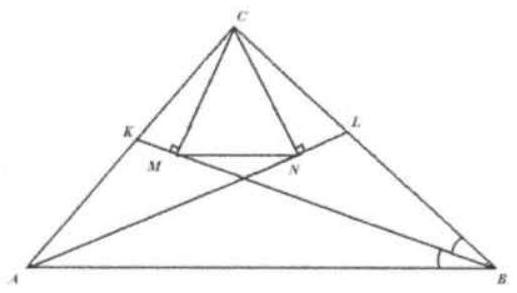
\includegraphics[width=\textwidth]{images/problem_image_1.jpg}

\section*{Solution}
Extend \(M N\) such that it intersects lines \(A C\) and \(B C\) at point \(O\) and \(Q\), respectively. Extend \(C M\) to meet \(A B\) at, say, \(S\). then triangle \(B C M\) and triangle \(B S M\) are congruent. Hence \(B S=B C=\) 120. Similarly, extend \(C N\) to meet \(A B\) at, say, \(R\), and triangle \(A C N\) and triangle \(A R N\) are congruent. Hence \(A R=A C\). So \(C M=M S\), and \(C N=N R\). So \(M N\) is the midline of triangle CSR.\\
\centering
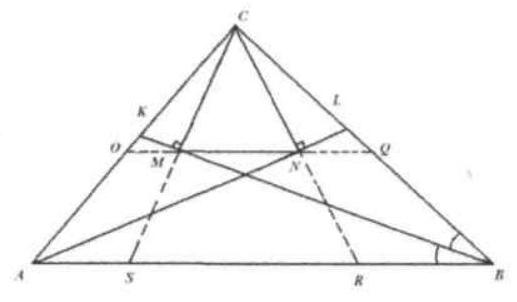
\includegraphics[width=\textwidth]{images/reasoning_image_1.jpg}


\(M N=\frac{S R}{2}\).\\
\(S R=A R-A S=A C-(A B-B S)=A C-(A B-B C)=B C+A C-A B\).\\
Thus \(M N=\frac{1}{2}(B C+A C-A B)\).

\end{document}
